\SourceLeaf{201}\begin{center}[2.]\end{center}


Es gibt viele solche Dinge, selbst in der Elementargeometrie, die eines strengen
Beweises bedürfen, z. B. die \textls{Möglichkeit der Ebene}, deren Definition eigentlich
schon ein Theorem involvirt; z. B. wenn $ABD$, $AFG$, $ACE$, $BFC$ gerade Linien
sind, dass dann die gerade Linie durch $DE$ nicht oberhalb oder unterhalb $G$
weggehen kann.

\begin{center}
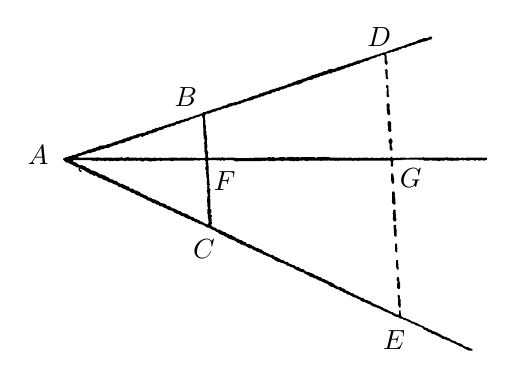
\begin{tikzpicture}[x=0.00627572cm,y=-0.00627572cm]
\fill[even odd rule] (776,563) -- (775,564) -- (775,567) -- (776,568) -- (776,573) -- (777,574) -- (776,576) -- (776,584) -- (777,585) -- (777,587) -- (779,589) -- (780,589) -- (781,588) -- (781,584) -- (782,583) -- (781,581) -- (781,572) -- (779,570) -- (780,568) -- (779,564) -- (778,563) -- cycle
(775,527) -- (773,531) -- (773,533) -- (775,536) -- (775,539) -- (774,540) -- (774,548) -- (776,551) -- (779,551) -- (780,550) -- (780,538) -- (779,537) -- (778,528) -- (777,527) -- cycle
(774,492) -- (772,494) -- (772,507) -- (773,508) -- (773,510) -- (775,512) -- (776,512) -- (777,511) -- (777,506) -- (776,505) -- (777,501) -- (776,500) -- (776,493) -- cycle
(771,459) -- (770,460) -- (770,474) -- (773,477) -- (774,477) -- (775,476) -- (774,474) -- (774,471) -- (775,470) -- (774,468) -- (774,460) -- (773,459) -- cycle
(768,421) -- (767,422) -- (768,442) -- (770,445) -- (772,445) -- (773,444) -- (773,430) -- (772,429) -- (772,422) -- (771,421) -- cycle
(768,390) -- (766,392) -- (766,396) -- (765,397) -- (765,399) -- (766,400) -- (766,406) -- (765,408) -- (766,409) -- (766,412) -- (768,414) -- (771,414) -- (773,411) -- (772,409) -- (772,405) -- (771,404) -- (772,400) -- (771,399) -- (771,392) -- (769,390) -- cycle
(766,353) -- (764,355) -- (764,371) -- (763,373) -- (764,374) -- (764,377) -- (767,380) -- (769,380) -- (771,378) -- (770,363) -- (769,362) -- (770,357) -- (768,355) -- (768,354) -- cycle
(763,317) -- (762,318) -- (762,332) -- (763,333) -- (763,336) -- (765,338) -- (766,338) -- (768,336) -- (768,326) -- (767,325) -- (767,321) -- (766,320) -- (766,318) -- (765,317) -- cycle
(760,246) -- (757,250) -- (757,254) -- (759,257) -- (759,268) -- (762,271) -- (763,271) -- (765,269) -- (764,263) -- (763,262) -- (763,257) -- (764,256) -- (765,251) -- (762,246) -- cycle
(757,211) -- (755,214) -- (755,220) -- (756,221) -- (756,230) -- (758,233) -- (760,233) -- (763,230) -- (762,228) -- (762,214) -- (759,211) -- cycle
(755,175) -- (753,177) -- (753,183) -- (754,184) -- (753,186) -- (753,189) -- (754,190) -- (754,195) -- (755,196) -- (755,198) -- (756,199) -- (758,199) -- (760,197) -- (759,186) -- (758,185) -- (759,183) -- (759,177) -- (757,175) -- cycle
(753,138) -- (752,139) -- (752,143) -- (754,146) -- (754,149) -- (753,150) -- (753,161) -- (754,162) -- (757,162) -- (758,161) -- (758,159) -- (757,158) -- (757,147) -- (756,146) -- (757,141) -- (755,138) -- cycle
(751,106) -- (750,107) -- (751,122) -- (752,123) -- (752,125) -- (753,126) -- (755,126) -- (756,125) -- (756,123) -- (755,122) -- (755,108) -- (753,106) -- cycle
(927,675) -- (927,674) -- (925,672) -- (921,671) -- (918,669) -- (913,668) -- (909,666) -- (904,662) -- (896,660) -- (894,658) -- (890,656) -- (888,656) -- (882,653) -- (880,651) -- (876,650) -- (874,648) -- (871,648) -- (863,644) -- (861,642) -- (857,641) -- (855,639) -- (853,639) -- (850,637) -- (847,637) -- (843,634) -- (839,633) -- (835,630) -- (830,629) -- (827,626) -- (823,625) -- (812,619) -- (810,619) -- (807,617) -- (804,617) -- (802,615) -- (796,612) -- (794,612) -- (791,610) -- (786,609) -- (782,605) -- (781,595) -- (780,594) -- (778,595) -- (778,602) -- (777,603) -- (773,603) -- (771,601) -- (769,601) -- (765,598) -- (763,598) -- (750,591) -- (748,591) -- (743,587) -- (741,587) -- (736,584) -- (733,584) -- (731,582) -- (729,582) -- (723,579) -- (720,576) -- (718,576) -- (712,573) -- (709,573) -- (705,569) -- (701,569) -- (699,567) -- (697,567) -- (693,564) -- (690,564) -- (685,560) -- (681,559) -- (674,555) -- (672,555) -- (666,550) -- (663,550) -- (660,547) -- (655,547) -- (648,543) -- (645,540) -- (639,537) -- (637,537) -- (633,534) -- (629,533) -- (627,531) -- (624,531) -- (619,527) -- (616,527) -- (612,524) -- (609,524) -- (605,521) -- (601,519) -- (599,519) -- (596,517) -- (590,516) -- (584,511) -- (581,511) -- (577,509) -- (575,507) -- (572,507) -- (568,505) -- (566,503) -- (561,502) -- (559,500) -- (556,500) -- (553,497) -- (551,496) -- (548,496) -- (544,493) -- (539,492) -- (535,489) -- (532,488) -- (530,486) -- (527,486) -- (522,482) -- (518,482) -- (511,478) -- (509,478) -- (507,476) -- (505,476) -- (499,471) -- (497,471) -- (494,469) -- (487,467) -- (483,464) -- (481,464) -- (478,461) -- (476,461) -- (475,460) -- (470,460) -- (467,456) -- (464,456) -- (462,454) -- (458,452) -- (456,452) -- (451,449) -- (449,449) -- (445,445) -- (443,445) -- (439,442) -- (436,442) -- (431,439) -- (429,439) -- (426,436) -- (421,435) -- (419,433) -- (417,433) -- (415,431) -- (411,431) -- (406,427) -- (402,426) -- (398,423) -- (398,420) -- (399,419) -- (398,405) -- (399,404) -- (399,402) -- (396,399) -- (396,398) -- (398,396) -- (398,391) -- (396,389) -- (396,369) -- (395,368) -- (395,365) -- (396,364) -- (395,362) -- (396,349) -- (394,347) -- (394,341) -- (395,339) -- (394,338) -- (394,330) -- (393,329) -- (392,296) -- (391,295) -- (391,292) -- (393,290) -- (409,290) -- (410,291) -- (412,290) -- (414,290) -- (415,291) -- (418,291) -- (419,290) -- (421,290) -- (422,291) -- (425,291) -- (426,290) -- (441,290) -- (442,291) -- (445,291) -- (448,293) -- (450,293) -- (451,292) -- (499,292) -- (500,291) -- (502,292) -- (504,291) -- (506,292) -- (508,291) -- (513,291) -- (514,292) -- (517,292) -- (518,291) -- (520,292) -- (527,292) -- (528,291) -- (539,291) -- (540,292) -- (543,292) -- (544,291) -- (556,291) -- (557,292) -- (560,291) -- (561,292) -- (567,292) -- (569,291) -- (570,292) -- (575,292) -- (576,291) -- (583,291) -- (584,290) -- (586,291) -- (589,291) -- (590,292) -- (593,292) -- (594,291) -- (618,291) -- (620,292) -- (621,291) -- (634,291) -- (635,290) -- (637,291) -- (647,291) -- (648,292) -- (650,291) -- (653,291) -- (654,292) -- (656,291) -- (683,291) -- (684,292) -- (686,291) -- (694,291) -- (696,292) -- (697,291) -- (756,291) -- (758,290) -- (762,294) -- (761,301) -- (763,303) -- (765,303) -- (766,302) -- (766,292) -- (768,290) -- (784,290) -- (785,289) -- (787,289) -- (788,290) -- (790,289) -- (818,289) -- (819,290) -- (821,290) -- (822,289) -- (824,289) -- (825,290) -- (828,290) -- (829,291) -- (840,291) -- (841,290) -- (843,290) -- (844,291) -- (856,291) -- (857,292) -- (860,292) -- (861,291) -- (870,291) -- (871,290) -- (875,290) -- (876,291) -- (884,291) -- (885,292) -- (887,291) -- (899,291) -- (900,290) -- (907,290) -- (908,291) -- (910,290) -- (914,290) -- (915,291) -- (921,291) -- (922,290) -- (929,290) -- (930,291) -- (933,291) -- (934,290) -- (938,290) -- (939,291) -- (948,290) -- (949,291) -- (951,291) -- (952,290) -- (955,290) -- (956,289) -- (956,286) -- (955,285) -- (951,285) -- (950,286) -- (948,285) -- (913,285) -- (912,286) -- (909,286) -- (908,285) -- (904,285) -- (903,286) -- (900,286) -- (899,285) -- (893,285) -- (892,286) -- (889,286) -- (888,285) -- (876,285) -- (875,284) -- (873,285) -- (845,285) -- (844,286) -- (842,285) -- (829,285) -- (828,284) -- (826,285) -- (799,285) -- (798,286) -- (793,286) -- (792,285) -- (780,285) -- (779,286) -- (773,285) -- (772,286) -- (766,286) -- (763,283) -- (762,283) -- (759,286) -- (756,286) -- (755,285) -- (752,285) -- (751,286) -- (748,286) -- (747,285) -- (741,285) -- (740,286) -- (733,286) -- (732,285) -- (730,286) -- (727,286) -- (726,285) -- (722,285) -- (721,286) -- (716,286) -- (715,285) -- (704,285) -- (703,286) -- (701,286) -- (700,285) -- (695,285) -- (694,286) -- (692,286) -- (691,285) -- (689,285) -- (688,286) -- (683,286) -- (682,285) -- (674,285) -- (673,286) -- (671,286) -- (670,285) -- (664,285) -- (662,286) -- (661,285) -- (656,285) -- (654,286) -- (653,285) -- (638,285) -- (637,284) -- (629,284) -- (628,283) -- (626,284) -- (613,284) -- (612,285) -- (608,285) -- (607,284) -- (579,284) -- (578,285) -- (576,285) -- (575,284) -- (569,284) -- (567,285) -- (566,284) -- (560,284) -- (558,283) -- (557,284) -- (552,284) -- (551,285) -- (547,285) -- (546,284) -- (536,284) -- (535,285) -- (529,285) -- (528,286) -- (527,286) -- (525,284) -- (521,284) -- (520,285) -- (518,285) -- (517,284) -- (513,284) -- (512,285) -- (498,285) -- (497,286) -- (495,285) -- (484,285) -- (483,286) -- (478,286) -- (477,285) -- (475,286) -- (447,286) -- (446,285) -- (429,285) -- (428,286) -- (426,286) -- (425,285) -- (422,285) -- (420,284) -- (419,285) -- (399,285) -- (398,286) -- (393,286) -- (391,284) -- (391,277) -- (392,275) -- (389,269) -- (389,267) -- (390,266) -- (389,264) -- (390,262) -- (390,259) -- (389,258) -- (389,249) -- (390,247) -- (389,246) -- (389,240) -- (388,239) -- (388,231) -- (386,229) -- (387,227) -- (387,220) -- (386,219) -- (386,209) -- (385,208) -- (385,199) -- (388,196) -- (394,196) -- (402,192) -- (406,192) -- (411,189) -- (417,188) -- (420,186) -- (423,186) -- (424,185) -- (429,185) -- (434,182) -- (439,181) -- (442,179) -- (448,179) -- (450,177) -- (454,177) -- (455,176) -- (457,176) -- (459,174) -- (461,174) -- (462,173) -- (464,173) -- (471,170) -- (479,169) -- (487,165) -- (490,165) -- (493,163) -- (496,163) -- (499,161) -- (503,161) -- (505,159) -- (507,159) -- (510,157) -- (518,156) -- (521,153) -- (525,153) -- (530,150) -- (535,150) -- (539,147) -- (543,147) -- (546,145) -- (549,145) -- (553,142) -- (557,142) -- (560,140) -- (565,139) -- (568,137) -- (574,137) -- (575,136) -- (577,136) -- (583,133) -- (585,131) -- (587,131) -- (594,128) -- (603,127) -- (606,124) -- (610,124) -- (611,123) -- (616,122) -- (618,120) -- (624,119) -- (627,117) -- (630,117) -- (636,114) -- (640,115) -- (644,112) -- (647,112) -- (654,109) -- (657,109) -- (663,106) -- (666,106) -- (670,103) -- (676,102) -- (682,99) -- (685,99) -- (687,97) -- (690,97) -- (694,95) -- (697,95) -- (702,92) -- (705,92) -- (707,90) -- (709,90) -- (710,89) -- (714,89) -- (721,85) -- (732,82) -- (734,80) -- (738,80) -- (743,77) -- (747,77) -- (749,79) -- (749,93) -- (750,95) -- (752,97) -- (753,97) -- (755,94) -- (755,91) -- (753,88) -- (753,79) -- (752,78) -- (752,75) -- (754,73) -- (758,73) -- (762,71) -- (767,71) -- (770,69) -- (776,68) -- (778,66) -- (781,66) -- (785,63) -- (787,63) -- (788,62) -- (791,63) -- (795,60) -- (797,60) -- (798,59) -- (802,59) -- (804,57) -- (810,56) -- (816,53) -- (820,53) -- (823,51) -- (825,51) -- (826,50) -- (830,50) -- (831,49) -- (836,48) -- (839,46) -- (843,46) -- (845,43) -- (845,41) -- (844,40) -- (840,40) -- (836,43) -- (827,43) -- (825,45) -- (819,46) -- (810,51) -- (807,51) -- (804,53) -- (800,53) -- (797,55) -- (790,57) -- (788,59) -- (784,59) -- (783,60) -- (772,63) -- (769,65) -- (766,65) -- (764,67) -- (758,68) -- (750,72) -- (746,72) -- (743,74) -- (740,74) -- (737,76) -- (734,76) -- (733,77) -- (731,77) -- (730,78) -- (728,78) -- (727,79) -- (725,79) -- (724,80) -- (722,80) -- (715,83) -- (712,83) -- (708,85) -- (705,85) -- (703,87) -- (701,87) -- (700,88) -- (695,88) -- (692,90) -- (689,90) -- (687,92) -- (685,92) -- (682,94) -- (678,94) -- (672,97) -- (669,97) -- (665,99) -- (662,99) -- (659,101) -- (656,101) -- (648,105) -- (636,106) -- (631,110) -- (626,110) -- (625,111) -- (623,111) -- (621,113) -- (618,113) -- (612,116) -- (609,116) -- (608,117) -- (602,118) -- (599,120) -- (592,122) -- (590,124) -- (584,125) -- (578,128) -- (574,128) -- (573,129) -- (571,129) -- (569,131) -- (566,131) -- (559,135) -- (555,135) -- (551,138) -- (549,138) -- (546,140) -- (542,140) -- (541,141) -- (536,142) -- (533,144) -- (529,144) -- (527,146) -- (523,146) -- (522,147) -- (517,148) -- (512,151) -- (509,151) -- (506,153) -- (503,153) -- (499,155) -- (496,155) -- (494,157) -- (490,159) -- (487,159) -- (486,160) -- (481,160) -- (479,162) -- (476,162) -- (474,164) -- (472,164) -- (470,166) -- (463,167) -- (460,169) -- (454,170) -- (452,172) -- (447,172) -- (443,174) -- (438,174) -- (437,175) -- (434,175) -- (428,179) -- (422,180) -- (416,183) -- (398,188) -- (395,190) -- (392,190) -- (385,193) -- (382,193) -- (378,196) -- (376,196) -- (373,198) -- (370,198) -- (369,199) -- (364,200) -- (361,202) -- (355,203) -- (349,206) -- (345,206) -- (342,208) -- (335,209) -- (332,211) -- (328,211) -- (324,214) -- (322,214) -- (318,216) -- (313,216) -- (311,218) -- (305,219) -- (302,221) -- (299,221) -- (297,223) -- (293,223) -- (290,225) -- (285,225) -- (283,227) -- (280,227) -- (276,230) -- (269,231) -- (263,235) -- (257,235) -- (256,236) -- (249,237) -- (243,240) -- (240,240) -- (238,242) -- (233,242) -- (231,244) -- (228,244) -- (225,246) -- (222,246) -- (214,250) -- (211,250) -- (208,252) -- (204,252) -- (201,254) -- (199,254) -- (197,256) -- (194,256) -- (193,257) -- (187,258) -- (183,260) -- (171,261) -- (168,264) -- (165,264) -- (164,265) -- (159,266) -- (156,268) -- (148,269) -- (144,272) -- (138,273) -- (134,276) -- (129,276) -- (123,279) -- (117,280) -- (113,282) -- (110,282) -- (107,284) -- (104,284) -- (98,287) -- (98,289) -- (104,295) -- (108,295) -- (112,298) -- (116,299) -- (120,302) -- (122,302) -- (125,305) -- (128,304) -- (129,305) -- (129,310) -- (132,314) -- (134,314) -- (135,313) -- (135,311) -- (133,311) -- (132,310) -- (132,308) -- (134,307) -- (138,310) -- (140,310) -- (143,313) -- (145,313) -- (147,315) -- (149,315) -- (152,318) -- (154,319) -- (157,319) -- (160,322) -- (164,321) -- (170,326) -- (176,327) -- (178,329) -- (182,331) -- (184,331) -- (188,333) -- (190,335) -- (194,335) -- (201,339) -- (206,340) -- (210,344) -- (214,344) -- (216,346) -- (222,349) -- (224,349) -- (228,352) -- (231,352) -- (238,357) -- (241,356) -- (245,360) -- (249,362) -- (252,362) -- (255,365) -- (257,365) -- (267,370) -- (269,372) -- (272,372) -- (280,377) -- (283,377) -- (287,380) -- (290,380) -- (293,383) -- (299,384) -- (303,387) -- (307,388) -- (311,391) -- (317,392) -- (321,394) -- (323,396) -- (329,399) -- (333,400) -- (337,403) -- (342,404) -- (346,407) -- (348,407) -- (350,409) -- (356,410) -- (359,413) -- (362,413) -- (365,416) -- (369,416) -- (373,419) -- (381,421) -- (390,427) -- (393,427) -- (399,430) -- (401,432) -- (404,432) -- (409,436) -- (411,436) -- (414,439) -- (420,442) -- (422,442) -- (426,445) -- (428,445) -- (430,447) -- (436,450) -- (443,452) -- (447,454) -- (450,457) -- (452,457) -- (456,459) -- (458,461) -- (461,461) -- (464,463) -- (467,463) -- (469,465) -- (476,469) -- (480,469) -- (484,473) -- (487,473) -- (489,475) -- (496,477) -- (498,479) -- (501,479) -- (504,482) -- (507,482) -- (509,484) -- (516,486) -- (520,488) -- (522,490) -- (524,490) -- (527,493) -- (533,496) -- (537,496) -- (539,498) -- (544,499) -- (550,502) -- (552,504) -- (555,504) -- (559,507) -- (562,507) -- (569,512) -- (573,514) -- (575,514) -- (577,516) -- (579,516) -- (580,517) -- (584,517) -- (587,520) -- (590,521) -- (592,523) -- (594,523) -- (596,525) -- (600,527) -- (603,527) -- (605,529) -- (610,530) -- (612,532) -- (614,532) -- (616,534) -- (618,534) -- (630,540) -- (632,540) -- (638,545) -- (642,547) -- (644,547) -- (653,552) -- (656,552) -- (659,555) -- (662,555) -- (664,557) -- (668,559) -- (670,559) -- (673,562) -- (679,563) -- (681,565) -- (687,568) -- (692,569) -- (694,571) -- (698,572) -- (701,575) -- (705,577) -- (709,577) -- (711,579) -- (721,583) -- (724,586) -- (727,586) -- (729,588) -- (732,588) -- (735,590) -- (737,590) -- (741,592) -- (743,594) -- (745,594) -- (752,598) -- (754,598) -- (759,601) -- (762,601) -- (765,604) -- (771,607) -- (777,608) -- (780,611) -- (784,611) -- (789,614) -- (794,615) -- (796,617) -- (800,618) -- (804,621) -- (807,621) -- (813,625) -- (816,625) -- (818,627) -- (821,627) -- (826,630) -- (829,634) -- (832,634) -- (837,638) -- (842,639) -- (845,642) -- (848,642) -- (862,649) -- (866,652) -- (872,653) -- (875,655) -- (880,656) -- (884,659) -- (888,660) -- (900,666) -- (902,668) -- (906,668) -- (908,670) -- (920,676) -- (926,676) -- cycle
(117,292) -- (119,290) -- (154,290) -- (155,291) -- (159,291) -- (160,292) -- (162,291) -- (164,291) -- (165,292) -- (167,292) -- (168,291) -- (175,291) -- (176,292) -- (178,291) -- (180,291) -- (181,292) -- (184,292) -- (185,291) -- (190,291) -- (191,292) -- (195,292) -- (196,291) -- (198,292) -- (200,292) -- (201,291) -- (203,291) -- (204,292) -- (211,292) -- (212,291) -- (221,291) -- (222,292) -- (224,292) -- (225,291) -- (230,291) -- (231,292) -- (233,291) -- (236,291) -- (237,292) -- (239,291) -- (245,291) -- (247,292) -- (248,291) -- (254,291) -- (255,292) -- (260,293) -- (263,291) -- (268,291) -- (269,292) -- (273,292) -- (274,293) -- (276,293) -- (277,292) -- (286,292) -- (287,291) -- (294,291) -- (295,292) -- (297,292) -- (298,291) -- (315,291) -- (316,292) -- (321,292) -- (322,291) -- (363,291) -- (364,290) -- (374,291) -- (375,290) -- (384,290) -- (387,293) -- (386,297) -- (388,302) -- (386,304) -- (386,309) -- (388,311) -- (387,318) -- (388,319) -- (388,325) -- (389,326) -- (389,340) -- (390,341) -- (390,344) -- (389,345) -- (390,347) -- (390,349) -- (389,350) -- (389,354) -- (390,355) -- (390,359) -- (391,360) -- (391,362) -- (390,363) -- (389,375) -- (390,376) -- (390,384) -- (391,385) -- (391,389) -- (390,390) -- (390,399) -- (391,400) -- (391,408) -- (392,409) -- (392,413) -- (393,414) -- (392,416) -- (392,419) -- (390,421) -- (388,419) -- (386,419) -- (382,417) -- (380,415) -- (376,414) -- (372,411) -- (370,411) -- (368,409) -- (365,409) -- (362,406) -- (355,404) -- (348,399) -- (339,397) -- (336,394) -- (334,393) -- (331,393) -- (327,390) -- (325,390) -- (323,388) -- (319,388) -- (316,385) -- (312,383) -- (309,383) -- (306,380) -- (302,378) -- (296,377) -- (289,372) -- (287,372) -- (284,370) -- (279,369) -- (275,366) -- (271,366) -- (268,363) -- (264,361) -- (262,361) -- (258,358) -- (256,358) -- (252,354) -- (250,354) -- (248,352) -- (245,352) -- (241,350) -- (239,348) -- (235,348) -- (233,347) -- (230,343) -- (227,343) -- (217,338) -- (214,338) -- (210,336) -- (206,332) -- (202,332) -- (197,329) -- (195,329) -- (191,327) -- (188,324) -- (186,324) -- (182,321) -- (180,321) -- (176,319) -- (173,319) -- (166,314) -- (164,314) -- (162,312) -- (158,312) -- (157,311) -- (155,311) -- (150,307) -- (146,306) -- (141,302) -- (139,302) -- (136,300) -- (131,300) -- (127,298) -- (124,295) -- (119,294) -- cycle
(381,205) -- (382,240) -- (383,241) -- (382,245) -- (384,247) -- (384,250) -- (385,251) -- (383,256) -- (384,257) -- (384,267) -- (385,268) -- (384,270) -- (384,273) -- (385,274) -- (385,278) -- (386,279) -- (386,284) -- (384,286) -- (367,286) -- (366,285) -- (363,285) -- (362,286) -- (360,286) -- (359,285) -- (355,285) -- (354,286) -- (352,286) -- (351,285) -- (337,285) -- (336,286) -- (334,285) -- (332,286) -- (330,286) -- (329,285) -- (312,285) -- (311,286) -- (307,286) -- (306,285) -- (304,286) -- (297,286) -- (296,285) -- (293,285) -- (292,286) -- (287,286) -- (286,285) -- (281,285) -- (280,286) -- (274,286) -- (273,285) -- (262,285) -- (261,286) -- (259,286) -- (258,285) -- (252,285) -- (251,286) -- (248,286) -- (247,285) -- (231,285) -- (230,284) -- (227,284) -- (226,285) -- (223,285) -- (222,286) -- (220,286) -- (216,284) -- (214,285) -- (202,285) -- (201,286) -- (199,286) -- (198,285) -- (179,285) -- (178,286) -- (176,286) -- (175,285) -- (169,285) -- (168,284) -- (166,285) -- (137,285) -- (136,286) -- (134,286) -- (133,285) -- (129,285) -- (128,284) -- (129,282) -- (131,282) -- (138,279) -- (141,279) -- (147,276) -- (154,276) -- (156,274) -- (160,274) -- (161,273) -- (163,273) -- (165,271) -- (172,270) -- (175,268) -- (180,268) -- (182,266) -- (191,265) -- (193,263) -- (198,262) -- (200,260) -- (204,260) -- (205,259) -- (207,259) -- (212,256) -- (217,256) -- (218,255) -- (221,255) -- (226,252) -- (232,251) -- (239,247) -- (248,245) -- (252,243) -- (254,241) -- (258,243) -- (266,239) -- (269,239) -- (273,236) -- (278,236) -- (281,234) -- (284,234) -- (291,230) -- (300,228) -- (302,226) -- (304,225) -- (307,225) -- (309,223) -- (314,223) -- (317,221) -- (324,220) -- (327,217) -- (335,216) -- (337,214) -- (343,213) -- (346,211) -- (351,211) -- (353,209) -- (359,206) -- (362,206) -- (368,203) -- (374,202) -- (376,200) -- (378,200) -- (380,202) -- (380,204) -- cycle;
\node[inner sep=0pt] at (738,41) {$D$};
\node[inner sep=0pt] at (346,162) {$B$};
\node[inner sep=0pt] at (47,280) {$A$};
\node[inner sep=0pt] at (425,332) {$F$};
\node[inner sep=0pt] at (802,327) {$G$};
\node[inner sep=0pt] at (383,470) {$C$};
\node[inner sep=0pt] at (768,655) {$E$};
\end{tikzpicture}

\end{center}

Der Beweis ist zwar nicht sehr schwer, aber doch auch nicht ganz leicht, und auf
jeden Fall in dieser oder einer andern Form unerlässlich.



\Needspace{9\baselineskip}
\begin{center}[3.]\end{center}


\begin{center}BEGRÜNDUNG DES PLANUM.\end{center}


1. \textls{Ebene} nennen wir die Fläche, in der jede durch einen gegebenen Punkt $A$
gehende Gerade $AD$ liegt, die mit der gegebenen Geraden $AB$ einen rechten
Winkel macht. Eine solche Ebene wird also beschrieben, wenn $AD$ sich um $AB$
als Axe dreht.

2. Wird $AB$ rückwärts nach $C$ fortgesetzt, so macht auch $AC$ mit jeder $AD$
rechte Winkel.

\begin{center}
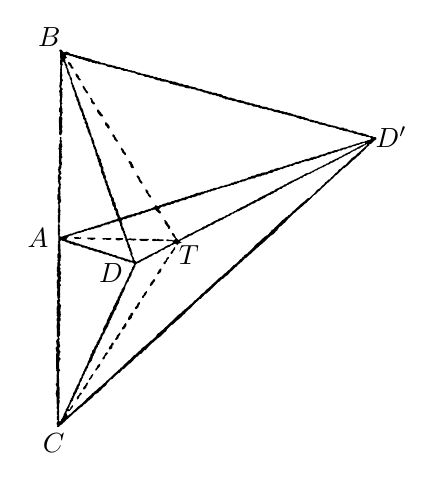
\begin{tikzpicture}[x=0.00572738cm,y=-0.00572738cm]
\fill[even odd rule] (790,265) -- (788,263) -- (784,263) -- (781,261) -- (775,261) -- (771,258) -- (769,258) -- (766,256) -- (763,256) -- (759,254) -- (748,253) -- (744,250) -- (741,250) -- (737,248) -- (733,249) -- (726,246) -- (724,244) -- (719,244) -- (717,242) -- (708,242) -- (702,239) -- (699,239) -- (698,238) -- (695,238) -- (694,237) -- (690,237) -- (686,235) -- (682,235) -- (676,232) -- (672,232) -- (668,230) -- (664,230) -- (658,227) -- (653,227) -- (650,225) -- (647,225) -- (646,224) -- (641,224) -- (639,222) -- (632,220) -- (629,218) -- (625,218) -- (621,216) -- (613,215) -- (610,213) -- (606,213) -- (603,211) -- (601,211) -- (597,209) -- (593,209) -- (591,207) -- (587,208) -- (584,206) -- (577,205) -- (574,203) -- (563,202) -- (562,201) -- (560,201) -- (558,199) -- (552,199) -- (546,196) -- (536,195) -- (535,194) -- (533,194) -- (531,192) -- (526,192) -- (525,191) -- (522,191) -- (515,188) -- (511,188) -- (507,186) -- (502,186) -- (499,184) -- (497,184) -- (493,182) -- (490,182) -- (489,181) -- (482,181) -- (474,177) -- (471,177) -- (467,175) -- (461,175) -- (455,172) -- (451,172) -- (446,168) -- (438,167) -- (435,165) -- (431,165) -- (430,164) -- (425,164) -- (422,162) -- (418,162) -- (417,161) -- (411,160) -- (410,159) -- (408,159) -- (401,156) -- (395,156) -- (387,152) -- (383,152) -- (382,151) -- (375,150) -- (373,148) -- (363,147) -- (358,144) -- (352,144) -- (349,142) -- (347,142) -- (343,140) -- (338,140) -- (334,138) -- (330,138) -- (326,136) -- (323,136) -- (322,135) -- (319,135) -- (318,134) -- (314,134) -- (311,132) -- (306,132) -- (301,129) -- (297,130) -- (293,127) -- (288,127) -- (285,125) -- (282,125) -- (281,124) -- (278,124) -- (277,123) -- (272,123) -- (271,122) -- (268,122) -- (265,120) -- (261,120) -- (252,116) -- (248,116) -- (247,115) -- (244,115) -- (243,114) -- (239,114) -- (237,112) -- (232,112) -- (229,110) -- (223,109) -- (222,108) -- (214,107) -- (208,104) -- (204,104) -- (203,103) -- (200,103) -- (199,102) -- (194,102) -- (187,99) -- (179,98) -- (174,95) -- (166,94) -- (165,93) -- (160,92) -- (155,89) -- (144,87) -- (140,85) -- (135,85) -- (133,83) -- (128,83) -- (124,81) -- (120,81) -- (117,79) -- (112,79) -- (110,77) -- (103,73) -- (96,75) -- (91,69) -- (87,69) -- (86,71) -- (88,74) -- (88,88) -- (89,89) -- (89,91) -- (88,92) -- (88,102) -- (89,103) -- (88,115) -- (89,117) -- (88,118) -- (88,126) -- (87,127) -- (88,129) -- (88,141) -- (87,142) -- (87,147) -- (86,148) -- (87,149) -- (86,150) -- (87,151) -- (87,154) -- (88,155) -- (88,157) -- (86,160) -- (86,163) -- (87,164) -- (87,171) -- (88,172) -- (88,179) -- (87,180) -- (87,185) -- (88,186) -- (88,195) -- (86,199) -- (86,207) -- (88,209) -- (88,211) -- (87,212) -- (88,216) -- (86,218) -- (86,220) -- (85,221) -- (85,230) -- (86,231) -- (86,236) -- (85,238) -- (86,239) -- (86,248) -- (87,249) -- (86,251) -- (86,256) -- (87,258) -- (89,259) -- (91,257) -- (92,253) -- (93,252) -- (93,248) -- (92,247) -- (92,243) -- (93,242) -- (93,237) -- (92,236) -- (93,220) -- (91,218) -- (91,216) -- (92,215) -- (92,212) -- (94,208) -- (93,207) -- (93,199) -- (92,198) -- (92,194) -- (91,193) -- (91,191) -- (93,189) -- (93,187) -- (91,185) -- (91,184) -- (92,183) -- (92,176) -- (93,175) -- (93,162) -- (92,161) -- (92,159) -- (94,157) -- (94,156) -- (91,153) -- (91,148) -- (92,147) -- (92,140) -- (94,138) -- (94,136) -- (92,133) -- (92,129) -- (93,128) -- (93,124) -- (92,123) -- (92,105) -- (94,102) -- (93,100) -- (93,96) -- (94,95) -- (96,96) -- (96,97) -- (98,99) -- (98,102) -- (100,105) -- (100,108) -- (102,110) -- (102,112) -- (103,113) -- (104,121) -- (109,129) -- (109,132) -- (112,138) -- (112,144) -- (114,147) -- (114,151) -- (116,153) -- (116,155) -- (120,163) -- (121,172) -- (124,176) -- (124,180) -- (127,185) -- (128,191) -- (131,196) -- (131,199) -- (137,211) -- (137,215) -- (139,218) -- (139,222) -- (143,227) -- (142,231) -- (146,236) -- (145,239) -- (149,247) -- (149,250) -- (151,253) -- (151,255) -- (153,257) -- (154,261) -- (156,264) -- (156,268) -- (158,271) -- (158,274) -- (161,280) -- (161,284) -- (163,286) -- (163,289) -- (165,291) -- (165,294) -- (166,295) -- (166,298) -- (167,299) -- (167,303) -- (170,307) -- (170,310) -- (172,314) -- (172,317) -- (174,320) -- (174,324) -- (175,325) -- (175,327) -- (178,330) -- (179,341) -- (183,349) -- (184,354) -- (186,356) -- (186,358) -- (187,359) -- (187,363) -- (189,366) -- (189,369) -- (191,371) -- (192,378) -- (194,381) -- (194,384) -- (196,386) -- (197,392) -- (199,394) -- (199,396) -- (201,399) -- (201,403) -- (203,407) -- (204,414) -- (208,419) -- (208,424) -- (211,427) -- (212,435) -- (215,439) -- (216,443) -- (214,445) -- (203,448) -- (200,450) -- (194,451) -- (193,452) -- (188,453) -- (185,455) -- (182,455) -- (176,458) -- (172,458) -- (171,459) -- (166,460) -- (163,462) -- (159,462) -- (156,464) -- (152,464) -- (150,466) -- (142,467) -- (140,469) -- (138,469) -- (134,471) -- (130,471) -- (129,472) -- (124,473) -- (121,475) -- (118,475) -- (115,477) -- (110,477) -- (108,479) -- (106,479) -- (102,481) -- (99,481) -- (92,484) -- (89,484) -- (87,482) -- (87,479) -- (88,478) -- (88,476) -- (87,475) -- (87,473) -- (88,472) -- (88,467) -- (87,466) -- (87,463) -- (88,462) -- (88,460) -- (87,459) -- (86,454) -- (88,451) -- (88,435) -- (89,434) -- (88,432) -- (89,425) -- (88,424) -- (88,414) -- (87,413) -- (87,411) -- (90,406) -- (90,402) -- (89,401) -- (89,394) -- (88,393) -- (88,391) -- (89,390) -- (88,379) -- (89,378) -- (89,370) -- (90,368) -- (89,367) -- (88,359) -- (91,354) -- (91,352) -- (88,349) -- (88,347) -- (91,344) -- (90,342) -- (90,339) -- (88,337) -- (88,336) -- (91,330) -- (91,325) -- (92,324) -- (92,319) -- (91,318) -- (91,310) -- (93,308) -- (93,306) -- (91,304) -- (92,302) -- (92,300) -- (91,299) -- (91,297) -- (92,296) -- (91,294) -- (91,292) -- (92,291) -- (91,287) -- (93,284) -- (92,278) -- (91,277) -- (92,271) -- (90,269) -- (91,267) -- (91,263) -- (88,263) -- (87,264) -- (88,266) -- (88,269) -- (87,270) -- (87,274) -- (88,276) -- (86,278) -- (86,280) -- (85,281) -- (85,287) -- (84,288) -- (86,292) -- (86,305) -- (85,306) -- (85,308) -- (86,309) -- (86,313) -- (85,314) -- (85,319) -- (86,320) -- (86,323) -- (87,325) -- (85,327) -- (85,329) -- (84,330) -- (84,334) -- (83,335) -- (84,337) -- (84,341) -- (85,342) -- (85,345) -- (83,348) -- (83,356) -- (84,357) -- (83,362) -- (84,363) -- (84,366) -- (85,367) -- (85,373) -- (83,376) -- (83,385) -- (84,386) -- (84,388) -- (82,391) -- (82,401) -- (84,404) -- (84,406) -- (83,407) -- (83,410) -- (84,411) -- (84,421) -- (83,422) -- (83,431) -- (84,432) -- (84,435) -- (83,436) -- (83,451) -- (84,452) -- (84,457) -- (83,458) -- (83,480) -- (84,481) -- (84,494) -- (83,495) -- (83,497) -- (84,498) -- (84,500) -- (83,501) -- (83,515) -- (84,516) -- (84,520) -- (82,523) -- (82,531) -- (83,532) -- (82,537) -- (83,538) -- (83,540) -- (82,541) -- (82,550) -- (81,551) -- (81,562) -- (82,563) -- (82,565) -- (81,566) -- (81,571) -- (82,572) -- (83,578) -- (81,581) -- (81,584) -- (80,585) -- (81,587) -- (81,598) -- (82,599) -- (81,614) -- (82,615) -- (82,620) -- (83,621) -- (83,624) -- (81,626) -- (82,637) -- (81,638) -- (81,641) -- (80,642) -- (80,647) -- (81,648) -- (81,650) -- (80,651) -- (81,657) -- (80,659) -- (82,661) -- (82,663) -- (80,667) -- (80,671) -- (82,673) -- (81,675) -- (81,679) -- (80,680) -- (80,687) -- (81,688) -- (81,705) -- (83,708) -- (83,710) -- (81,712) -- (79,716) -- (81,727) -- (78,731) -- (78,733) -- (79,734) -- (79,738) -- (80,739) -- (80,743) -- (79,744) -- (79,777) -- (80,779) -- (79,781) -- (81,783) -- (81,789) -- (80,790) -- (80,795) -- (81,796) -- (80,798) -- (80,809) -- (78,811) -- (81,819) -- (80,820) -- (80,825) -- (79,826) -- (79,830) -- (78,831) -- (78,833) -- (79,834) -- (79,838) -- (80,839) -- (80,854) -- (81,855) -- (81,861) -- (80,862) -- (80,864) -- (82,868) -- (82,870) -- (81,871) -- (81,879) -- (82,880) -- (82,882) -- (81,883) -- (81,890) -- (83,892) -- (80,898) -- (80,900) -- (82,902) -- (81,906) -- (85,906) -- (89,902) -- (93,900) -- (94,898) -- (96,896) -- (97,896) -- (103,889) -- (104,889) -- (110,883) -- (111,883) -- (120,874) -- (121,874) -- (133,863) -- (137,861) -- (141,856) -- (144,855) -- (152,847) -- (153,847) -- (157,843) -- (158,843) -- (165,834) -- (173,830) -- (174,828) -- (176,826) -- (177,826) -- (184,818) -- (185,818) -- (191,813) -- (191,811) -- (200,801) -- (205,799) -- (206,797) -- (213,790) -- (214,790) -- (218,786) -- (220,786) -- (227,778) -- (229,778) -- (241,766) -- (244,765) -- (258,750) -- (260,750) -- (265,744) -- (268,744) -- (275,736) -- (277,736) -- (280,733) -- (280,732) -- (282,731) -- (282,730) -- (293,719) -- (294,719) -- (305,709) -- (310,706) -- (321,695) -- (322,695) -- (324,693) -- (325,690) -- (335,680) -- (338,679) -- (348,669) -- (349,669) -- (356,663) -- (357,663) -- (358,661) -- (363,656) -- (364,656) -- (366,654) -- (366,653) -- (374,645) -- (375,645) -- (390,629) -- (391,629) -- (398,622) -- (400,622) -- (410,611) -- (413,610) -- (419,604) -- (420,604) -- (422,602) -- (422,601) -- (424,599) -- (425,599) -- (440,584) -- (441,584) -- (446,579) -- (450,577) -- (455,572) -- (459,570) -- (468,560) -- (469,560) -- (478,551) -- (479,551) -- (484,545) -- (485,545) -- (489,541) -- (490,541) -- (498,532) -- (502,530) -- (509,523) -- (510,523) -- (518,515) -- (519,515) -- (526,508) -- (527,508) -- (534,501) -- (535,501) -- (556,481) -- (558,481) -- (560,479) -- (561,479) -- (566,474) -- (566,473) -- (571,469) -- (571,467) -- (573,465) -- (573,464) -- (576,461) -- (578,461) -- (585,454) -- (586,454) -- (596,442) -- (597,442) -- (608,431) -- (609,431) -- (616,424) -- (617,424) -- (618,422) -- (619,422) -- (623,418) -- (624,418) -- (631,411) -- (635,409) -- (636,407) -- (641,402) -- (642,402) -- (651,392) -- (655,390) -- (663,382) -- (664,382) -- (670,375) -- (671,375) -- (682,364) -- (683,364) -- (692,355) -- (693,355) -- (699,348) -- (703,346) -- (717,332) -- (719,332) -- (723,328) -- (724,328) -- (738,314) -- (742,312) -- (749,305) -- (750,305) -- (756,299) -- (756,298) -- (759,295) -- (760,295) -- (768,287) -- (768,286) -- (774,281) -- (774,280) -- (776,278) -- (778,278) -- (786,270) -- (787,270) -- (790,267) -- cycle
(91,491) -- (93,493) -- (98,494) -- (104,497) -- (107,497) -- (110,500) -- (115,500) -- (119,503) -- (130,504) -- (131,505) -- (133,505) -- (137,508) -- (142,508) -- (145,510) -- (148,510) -- (153,513) -- (157,513) -- (166,517) -- (171,517) -- (172,518) -- (174,518) -- (176,520) -- (180,520) -- (186,523) -- (194,524) -- (199,527) -- (203,527) -- (206,529) -- (209,529) -- (214,532) -- (222,533) -- (224,535) -- (227,535) -- (234,539) -- (239,539) -- (242,541) -- (248,541) -- (252,544) -- (252,546) -- (250,550) -- (248,552) -- (248,555) -- (246,557) -- (246,560) -- (242,565) -- (240,572) -- (237,576) -- (237,578) -- (233,585) -- (233,587) -- (231,589) -- (231,591) -- (229,595) -- (224,602) -- (224,605) -- (222,607) -- (220,611) -- (220,613) -- (216,619) -- (215,624) -- (213,626) -- (212,630) -- (210,632) -- (209,635) -- (206,639) -- (205,645) -- (203,649) -- (199,654) -- (198,658) -- (196,660) -- (196,662) -- (192,670) -- (191,675) -- (189,677) -- (189,679) -- (187,681) -- (183,689) -- (183,695) -- (178,701) -- (177,706) -- (174,710) -- (174,712) -- (171,715) -- (171,717) -- (169,719) -- (169,722) -- (164,729) -- (163,733) -- (159,737) -- (159,740) -- (157,744) -- (155,746) -- (155,750) -- (153,753) -- (152,758) -- (150,760) -- (148,767) -- (146,771) -- (144,773) -- (144,775) -- (142,778) -- (141,782) -- (139,784) -- (139,786) -- (136,791) -- (135,796) -- (133,798) -- (131,802) -- (131,804) -- (129,807) -- (129,809) -- (126,813) -- (124,817) -- (124,819) -- (122,821) -- (122,823) -- (120,825) -- (120,827) -- (117,831) -- (116,837) -- (114,839) -- (114,841) -- (112,843) -- (112,845) -- (110,847) -- (109,852) -- (103,864) -- (100,868) -- (100,871) -- (96,878) -- (96,880) -- (92,888) -- (90,890) -- (90,892) -- (88,894) -- (87,894) -- (85,892) -- (86,890) -- (86,880) -- (85,879) -- (85,876) -- (86,875) -- (86,869) -- (85,868) -- (85,864) -- (86,863) -- (86,854) -- (87,853) -- (87,847) -- (86,846) -- (86,844) -- (87,843) -- (87,837) -- (86,836) -- (87,834) -- (87,828) -- (86,827) -- (87,825) -- (87,819) -- (86,818) -- (86,814) -- (85,813) -- (86,811) -- (85,787) -- (86,786) -- (86,783) -- (88,781) -- (88,780) -- (86,777) -- (86,773) -- (85,772) -- (86,770) -- (86,766) -- (85,764) -- (86,763) -- (87,758) -- (89,756) -- (89,754) -- (86,751) -- (86,749) -- (87,748) -- (87,743) -- (89,739) -- (87,737) -- (87,735) -- (86,734) -- (86,731) -- (88,727) -- (88,724) -- (87,723) -- (87,718) -- (85,715) -- (85,714) -- (87,712) -- (87,710) -- (85,708) -- (85,707) -- (88,702) -- (88,694) -- (87,693) -- (88,678) -- (87,677) -- (87,672) -- (89,670) -- (89,665) -- (88,664) -- (88,662) -- (89,661) -- (89,658) -- (90,657) -- (89,655) -- (89,650) -- (88,649) -- (90,636) -- (88,634) -- (86,629) -- (88,627) -- (88,624) -- (87,623) -- (87,620) -- (88,619) -- (88,608) -- (87,606) -- (88,605) -- (88,594) -- (90,592) -- (87,586) -- (87,585) -- (90,582) -- (89,580) -- (90,573) -- (88,571) -- (90,567) -- (90,562) -- (88,560) -- (89,554) -- (87,551) -- (87,550) -- (89,548) -- (89,545) -- (88,544) -- (88,538) -- (89,537) -- (89,531) -- (90,530) -- (90,525) -- (89,524) -- (89,519) -- (88,518) -- (89,516) -- (88,494) -- cycle
(249,536) -- (248,537) -- (244,537) -- (242,535) -- (239,535) -- (236,533) -- (233,533) -- (226,530) -- (222,530) -- (221,529) -- (216,528) -- (212,525) -- (206,525) -- (202,522) -- (199,522) -- (195,520) -- (192,520) -- (186,517) -- (183,517) -- (177,514) -- (170,513) -- (167,511) -- (164,511) -- (160,509) -- (156,509) -- (153,507) -- (151,507) -- (147,505) -- (144,505) -- (141,503) -- (138,503) -- (137,502) -- (132,501) -- (129,499) -- (125,499) -- (117,495) -- (113,495) -- (112,494) -- (104,492) -- (102,490) -- (102,489) -- (108,482) -- (115,481) -- (118,479) -- (123,478) -- (126,476) -- (134,475) -- (135,474) -- (140,473) -- (143,471) -- (146,471) -- (149,469) -- (154,469) -- (158,467) -- (163,467) -- (165,465) -- (168,465) -- (169,464) -- (172,464) -- (173,463) -- (177,463) -- (183,459) -- (186,459) -- (189,457) -- (192,457) -- (193,456) -- (196,457) -- (198,455) -- (202,453) -- (206,453) -- (212,450) -- (215,450) -- (217,449) -- (219,451) -- (221,455) -- (221,459) -- (223,462) -- (224,468) -- (227,472) -- (227,474) -- (229,477) -- (229,480) -- (231,483) -- (231,486) -- (233,488) -- (233,492) -- (236,497) -- (236,500) -- (238,503) -- (238,507) -- (241,511) -- (241,514) -- (244,519) -- (244,524) -- (247,529) -- cycle
(211,488) -- (211,490) -- (214,492) -- (221,492) -- (222,491) -- (226,491) -- (228,489) -- (227,487) -- (212,487) -- cycle
(182,488) -- (182,489) -- (185,491) -- (187,490) -- (190,490) -- (191,491) -- (199,491) -- (202,489) -- (201,487) -- (183,487) -- cycle
(148,487) -- (149,489) -- (151,490) -- (154,489) -- (156,491) -- (161,491) -- (162,490) -- (165,490) -- (166,489) -- (166,487) -- (165,486) -- (149,486) -- cycle
(119,486) -- (119,487) -- (122,489) -- (132,489) -- (135,487) -- (134,485) -- (132,486) -- (130,486) -- (129,485) -- (120,485) -- cycle
(770,280) -- (749,299) -- (748,299) -- (744,304) -- (736,309) -- (721,325) -- (718,326) -- (711,333) -- (708,334) -- (705,337) -- (705,338) -- (701,342) -- (700,342) -- (691,352) -- (690,352) -- (688,354) -- (688,355) -- (686,357) -- (684,357) -- (678,363) -- (677,363) -- (675,365) -- (675,366) -- (671,370) -- (670,370) -- (665,376) -- (660,379) -- (655,384) -- (655,385) -- (641,398) -- (637,399) -- (630,406) -- (629,406) -- (625,410) -- (624,410) -- (615,419) -- (614,419) -- (607,426) -- (606,426) -- (598,435) -- (595,436) -- (592,440) -- (590,440) -- (585,445) -- (580,448) -- (579,450) -- (567,462) -- (566,462) -- (561,468) -- (558,469) -- (556,471) -- (556,472) -- (548,481) -- (546,481) -- (544,483) -- (543,483) -- (527,498) -- (526,498) -- (521,503) -- (520,503) -- (518,507) -- (512,513) -- (511,513) -- (510,515) -- (508,517) -- (507,517) -- (503,522) -- (501,522) -- (499,524) -- (498,524) -- (496,526) -- (496,527) -- (494,529) -- (493,529) -- (492,531) -- (490,533) -- (489,533) -- (480,543) -- (479,543) -- (476,546) -- (473,547) -- (463,558) -- (462,558) -- (455,565) -- (454,565) -- (446,573) -- (444,573) -- (426,590) -- (425,590) -- (424,592) -- (415,600) -- (414,600) -- (407,608) -- (402,611) -- (394,620) -- (393,620) -- (388,625) -- (387,625) -- (380,633) -- (379,633) -- (366,645) -- (365,645) -- (361,649) -- (360,649) -- (356,654) -- (352,656) -- (323,684) -- (322,684) -- (316,691) -- (315,691) -- (307,698) -- (306,698) -- (303,701) -- (301,705) -- (296,710) -- (295,710) -- (292,714) -- (290,714) -- (282,722) -- (281,722) -- (276,727) -- (271,730) -- (267,734) -- (267,735) -- (265,737) -- (264,737) -- (255,746) -- (252,747) -- (242,758) -- (241,758) -- (234,765) -- (233,765) -- (225,774) -- (222,775) -- (221,777) -- (219,779) -- (218,779) -- (214,784) -- (213,784) -- (193,803) -- (192,803) -- (187,809) -- (186,809) -- (179,816) -- (174,819) -- (167,826) -- (166,826) -- (161,831) -- (160,831) -- (154,838) -- (153,838) -- (149,842) -- (148,842) -- (146,844) -- (146,845) -- (135,856) -- (134,856) -- (130,860) -- (129,860) -- (110,878) -- (109,878) -- (106,881) -- (104,881) -- (103,880) -- (102,873) -- (104,871) -- (109,871) -- (117,861) -- (117,859) -- (115,858) -- (111,863) -- (111,865) -- (108,868) -- (106,866) -- (109,861) -- (109,859) -- (111,857) -- (111,855) -- (113,851) -- (116,848) -- (118,841) -- (123,831) -- (125,829) -- (125,827) -- (127,823) -- (129,821) -- (129,817) -- (132,813) -- (132,809) -- (136,803) -- (136,800) -- (139,797) -- (139,793) -- (141,791) -- (143,787) -- (143,785) -- (146,782) -- (147,778) -- (150,774) -- (150,772) -- (153,765) -- (159,758) -- (159,755) -- (160,754) -- (161,749) -- (163,747) -- (163,745) -- (166,741) -- (167,736) -- (170,730) -- (172,728) -- (172,725) -- (175,722) -- (175,720) -- (177,718) -- (177,715) -- (179,713) -- (181,709) -- (181,707) -- (184,701) -- (186,699) -- (190,689) -- (193,686) -- (193,684) -- (195,682) -- (195,679) -- (198,675) -- (198,671) -- (201,668) -- (201,666) -- (204,661) -- (204,659) -- (207,655) -- (207,653) -- (209,649) -- (213,645) -- (213,641) -- (217,633) -- (219,631) -- (219,627) -- (220,626) -- (221,621) -- (223,619) -- (223,617) -- (226,613) -- (226,610) -- (228,608) -- (232,600) -- (233,594) -- (237,586) -- (240,583) -- (241,578) -- (246,571) -- (247,565) -- (249,562) -- (249,560) -- (253,555) -- (253,553) -- (255,550) -- (255,547) -- (259,543) -- (265,541) -- (270,537) -- (272,537) -- (274,535) -- (276,535) -- (278,533) -- (280,533) -- (288,528) -- (290,528) -- (296,523) -- (298,522) -- (301,522) -- (305,520) -- (307,518) -- (310,517) -- (313,514) -- (316,514) -- (320,512) -- (323,509) -- (331,506) -- (336,502) -- (338,502) -- (343,499) -- (348,502) -- (350,501) -- (351,499) -- (354,499) -- (356,497) -- (359,496) -- (356,496) -- (354,494) -- (356,492) -- (373,484) -- (375,482) -- (380,481) -- (387,476) -- (403,468) -- (406,468) -- (408,466) -- (412,464) -- (414,464) -- (417,461) -- (420,460) -- (422,458) -- (425,458) -- (429,456) -- (435,451) -- (440,450) -- (445,447) -- (449,446) -- (452,443) -- (454,443) -- (458,440) -- (462,438) -- (464,438) -- (470,433) -- (473,433) -- (476,430) -- (478,430) -- (481,428) -- (486,427) -- (488,425) -- (490,425) -- (492,423) -- (503,418) -- (506,415) -- (508,415) -- (514,411) -- (519,410) -- (525,405) -- (528,405) -- (532,403) -- (534,401) -- (536,401) -- (538,399) -- (542,398) -- (548,393) -- (550,393) -- (552,391) -- (555,391) -- (557,389) -- (561,388) -- (564,385) -- (568,384) -- (571,381) -- (576,378) -- (579,378) -- (583,374) -- (589,372) -- (592,369) -- (594,369) -- (598,366) -- (600,366) -- (604,363) -- (606,363) -- (609,360) -- (611,360) -- (619,356) -- (621,354) -- (625,354) -- (630,349) -- (633,349) -- (637,346) -- (644,344) -- (647,341) -- (650,341) -- (653,338) -- (655,337) -- (658,337) -- (660,335) -- (670,330) -- (672,330) -- (674,328) -- (676,328) -- (678,326) -- (682,324) -- (684,324) -- (690,320) -- (694,319) -- (701,314) -- (704,314) -- (708,310) -- (710,310) -- (714,308) -- (716,306) -- (718,306) -- (720,304) -- (724,303) -- (728,300) -- (730,300) -- (735,296) -- (741,293) -- (743,293) -- (748,289) -- (753,288) -- (756,285) -- (759,284) -- (763,281) -- (765,281) -- (768,278) -- cycle
(134,830) -- (133,830) -- (131,832) -- (131,834) -- (126,839) -- (125,841) -- (125,845) -- (127,845) -- (130,842) -- (131,838) -- (136,833) -- (136,832) -- cycle
(149,808) -- (147,808) -- (143,815) -- (140,818) -- (139,820) -- (139,822) -- (140,823) -- (142,823) -- (146,819) -- (146,817) -- (149,813) -- (149,811) -- (150,810) -- cycle
(161,789) -- (160,789) -- (156,793) -- (155,796) -- (152,799) -- (152,801) -- (153,802) -- (154,802) -- (159,796) -- (160,793) -- (162,791) -- cycle
(176,766) -- (175,766) -- (170,771) -- (169,775) -- (166,778) -- (166,780) -- (167,781) -- (168,781) -- (176,772) -- (177,770) -- (177,767) -- cycle
(193,741) -- (190,741) -- (188,743) -- (186,748) -- (182,753) -- (182,755) -- (183,756) -- (185,756) -- (187,754) -- (188,750) -- (194,743) -- cycle
(205,719) -- (204,719) -- (202,721) -- (201,724) -- (196,730) -- (196,733) -- (197,734) -- (200,734) -- (203,732) -- (204,730) -- (204,726) -- (207,723) -- (207,721) -- cycle
(221,697) -- (220,697) -- (214,703) -- (213,707) -- (210,711) -- (211,713) -- (213,713) -- (217,710) -- (218,706) -- (222,700) -- (222,698) -- cycle
(234,676) -- (233,676) -- (230,679) -- (228,683) -- (225,686) -- (225,689) -- (226,690) -- (230,689) -- (235,682) -- (235,677) -- cycle
(249,653) -- (246,653) -- (244,655) -- (244,657) -- (240,661) -- (240,663) -- (239,664) -- (239,668) -- (240,669) -- (243,668) -- (247,664) -- (247,660) -- (250,657) -- (250,654) -- cycle
(264,629) -- (263,629) -- (260,632) -- (258,637) -- (254,641) -- (254,643) -- (256,645) -- (257,645) -- (262,640) -- (262,638) -- (265,633) -- (265,630) -- cycle
(280,605) -- (279,605) -- (274,610) -- (274,612) -- (270,616) -- (270,619) -- (271,620) -- (273,620) -- (275,616) -- (278,613) -- (281,607) -- cycle
(297,578) -- (295,579) -- (290,585) -- (287,591) -- (288,593) -- (290,593) -- (294,589) -- (295,586) -- (299,582) -- (299,580) -- cycle
(312,555) -- (310,555) -- (307,558) -- (305,563) -- (303,565) -- (304,567) -- (306,567) -- (311,563) -- (313,559) -- (313,556) -- cycle
(329,529) -- (327,529) -- (324,532) -- (323,536) -- (317,542) -- (317,543) -- (319,545) -- (321,545) -- (322,544) -- (322,542) -- (325,539) -- (326,535) -- (330,531) -- cycle
(343,507) -- (341,508) -- (339,512) -- (333,519) -- (333,521) -- (334,522) -- (336,522) -- (339,519) -- (339,517) -- (343,512) -- cycle
(765,276) -- (765,278) -- (764,279) -- (762,279) -- (748,286) -- (746,288) -- (744,288) -- (742,290) -- (740,290) -- (738,292) -- (734,293) -- (732,295) -- (721,300) -- (719,302) -- (717,302) -- (712,306) -- (709,306) -- (707,308) -- (701,311) -- (699,311) -- (697,313) -- (694,314) -- (690,317) -- (687,317) -- (683,321) -- (680,321) -- (677,324) -- (675,324) -- (671,326) -- (669,328) -- (667,328) -- (665,330) -- (662,330) -- (658,333) -- (653,335) -- (651,337) -- (649,337) -- (647,339) -- (643,340) -- (641,342) -- (635,343) -- (631,345) -- (629,347) -- (626,348) -- (624,350) -- (622,350) -- (618,353) -- (616,353) -- (614,355) -- (612,355) -- (610,357) -- (608,357) -- (606,359) -- (604,359) -- (594,364) -- (592,366) -- (588,368) -- (586,368) -- (583,371) -- (581,371) -- (579,373) -- (577,373) -- (575,375) -- (567,378) -- (563,382) -- (556,384) -- (554,386) -- (540,393) -- (538,393) -- (536,395) -- (529,398) -- (526,401) -- (522,403) -- (520,403) -- (518,405) -- (516,405) -- (514,407) -- (509,409) -- (507,411) -- (503,412) -- (499,415) -- (487,420) -- (485,422) -- (483,422) -- (477,427) -- (475,427) -- (471,430) -- (465,432) -- (460,436) -- (458,436) -- (454,438) -- (452,440) -- (450,440) -- (447,442) -- (440,444) -- (437,447) -- (435,447) -- (427,451) -- (420,456) -- (418,456) -- (412,459) -- (410,461) -- (407,461) -- (400,466) -- (392,470) -- (390,470) -- (386,473) -- (376,478) -- (374,478) -- (370,480) -- (368,482) -- (366,482) -- (363,485) -- (360,486) -- (358,488) -- (356,488) -- (352,491) -- (350,491) -- (345,486) -- (342,479) -- (339,476) -- (337,476) -- (336,478) -- (338,482) -- (344,488) -- (344,489) -- (340,492) -- (338,492) -- (337,491) -- (329,491) -- (328,490) -- (325,490) -- (324,491) -- (324,493) -- (325,494) -- (337,494) -- (339,496) -- (336,499) -- (331,502) -- (329,502) -- (321,506) -- (316,510) -- (314,510) -- (312,512) -- (310,512) -- (308,514) -- (306,514) -- (303,517) -- (301,517) -- (297,520) -- (293,521) -- (283,526) -- (281,528) -- (277,529) -- (275,531) -- (271,533) -- (269,533) -- (267,535) -- (257,540) -- (252,535) -- (252,532) -- (248,525) -- (249,520) -- (247,518) -- (246,512) -- (243,506) -- (243,503) -- (240,499) -- (240,497) -- (239,496) -- (239,492) -- (240,491) -- (244,491) -- (245,492) -- (249,492) -- (251,493) -- (252,492) -- (255,492) -- (257,491) -- (257,490) -- (255,488) -- (245,488) -- (243,487) -- (242,488) -- (238,489) -- (236,487) -- (235,481) -- (232,476) -- (232,472) -- (230,470) -- (230,467) -- (226,460) -- (226,454) -- (224,449) -- (228,445) -- (234,445) -- (238,442) -- (246,441) -- (248,439) -- (250,439) -- (251,438) -- (254,439) -- (259,435) -- (266,435) -- (270,432) -- (276,431) -- (279,429) -- (282,429) -- (285,427) -- (288,427) -- (290,425) -- (294,425) -- (295,424) -- (299,424) -- (301,426) -- (301,427) -- (302,427) -- (305,430) -- (310,433) -- (312,429) -- (308,425) -- (308,422) -- (311,419) -- (315,417) -- (320,417) -- (325,414) -- (333,413) -- (335,411) -- (339,411) -- (343,408) -- (349,408) -- (356,404) -- (359,404) -- (360,403) -- (365,403) -- (374,398) -- (379,398) -- (382,396) -- (386,396) -- (387,395) -- (389,395) -- (394,392) -- (399,392) -- (401,390) -- (404,390) -- (411,386) -- (415,386) -- (418,384) -- (422,384) -- (425,382) -- (431,381) -- (437,378) -- (440,378) -- (447,375) -- (458,373) -- (461,371) -- (465,371) -- (468,369) -- (473,369) -- (475,367) -- (479,367) -- (482,365) -- (484,365) -- (486,363) -- (490,363) -- (493,361) -- (497,361) -- (505,357) -- (509,357) -- (512,355) -- (515,355) -- (516,354) -- (519,355) -- (524,351) -- (533,350) -- (536,348) -- (539,348) -- (542,346) -- (547,346) -- (551,343) -- (559,342) -- (562,339) -- (564,339) -- (565,338) -- (569,338) -- (572,336) -- (576,335) -- (578,333) -- (582,334) -- (584,332) -- (586,332) -- (589,330) -- (591,330) -- (592,329) -- (596,329) -- (598,327) -- (603,327) -- (607,325) -- (609,323) -- (618,322) -- (619,321) -- (621,321) -- (623,319) -- (629,318) -- (631,316) -- (640,316) -- (643,314) -- (650,313) -- (652,311) -- (656,311) -- (658,309) -- (662,309) -- (670,305) -- (675,305) -- (682,301) -- (686,301) -- (692,298) -- (695,298) -- (699,296) -- (702,296) -- (707,293) -- (712,293) -- (716,290) -- (721,290) -- (728,286) -- (733,286) -- (738,283) -- (741,283) -- (748,280) -- (751,280) -- (754,278) -- (756,278) -- (763,275) -- cycle
(292,491) -- (293,493) -- (295,493) -- (296,494) -- (298,494) -- (299,493) -- (307,493) -- (308,494) -- (312,494) -- (313,493) -- (317,493) -- (318,492) -- (317,490) -- (308,490) -- (307,489) -- (304,489) -- (303,490) -- (301,490) -- (300,489) -- (294,489) -- cycle
(264,490) -- (264,491) -- (267,493) -- (281,493) -- (285,491) -- (284,489) -- (265,489) -- cycle
(320,447) -- (319,448) -- (320,450) -- (320,454) -- (327,463) -- (327,465) -- (329,467) -- (330,467) -- (332,465) -- (332,461) -- (327,455) -- (326,452) -- (321,447) -- cycle
(100,82) -- (102,80) -- (103,81) -- (107,81) -- (111,83) -- (115,83) -- (118,85) -- (121,85) -- (123,87) -- (126,87) -- (130,89) -- (137,90) -- (140,92) -- (143,92) -- (144,93) -- (149,94) -- (152,96) -- (156,95) -- (160,98) -- (164,98) -- (167,100) -- (171,99) -- (173,101) -- (184,102) -- (185,103) -- (188,103) -- (194,107) -- (204,108) -- (210,111) -- (222,112) -- (224,114) -- (226,114) -- (229,116) -- (236,116) -- (237,117) -- (243,118) -- (247,120) -- (252,120) -- (262,125) -- (268,125) -- (269,126) -- (272,126) -- (276,129) -- (281,129) -- (282,130) -- (285,130) -- (288,132) -- (294,132) -- (301,136) -- (303,136) -- (304,137) -- (309,137) -- (312,139) -- (315,139) -- (316,140) -- (323,140) -- (324,141) -- (328,141) -- (333,145) -- (337,145) -- (338,146) -- (344,147) -- (345,148) -- (350,148) -- (353,150) -- (362,151) -- (367,154) -- (371,154) -- (372,155) -- (379,155) -- (380,156) -- (388,157) -- (391,159) -- (393,159) -- (394,160) -- (398,160) -- (399,161) -- (404,162) -- (407,164) -- (412,164) -- (414,166) -- (416,166) -- (420,168) -- (425,168) -- (427,170) -- (433,170) -- (436,172) -- (440,172) -- (443,174) -- (446,174) -- (450,177) -- (453,177) -- (455,179) -- (461,179) -- (462,180) -- (468,181) -- (472,183) -- (478,183) -- (484,186) -- (496,188) -- (499,190) -- (502,190) -- (506,192) -- (512,192) -- (517,195) -- (526,196) -- (532,199) -- (536,199) -- (537,200) -- (540,200) -- (541,201) -- (546,201) -- (550,203) -- (555,203) -- (564,207) -- (572,208) -- (573,209) -- (577,209) -- (582,212) -- (587,212) -- (588,213) -- (592,213) -- (596,215) -- (600,215) -- (601,216) -- (608,217) -- (609,218) -- (611,218) -- (615,221) -- (617,221) -- (621,223) -- (625,222) -- (631,225) -- (635,225) -- (636,226) -- (641,227) -- (643,229) -- (646,229) -- (647,230) -- (652,230) -- (655,232) -- (659,232) -- (664,235) -- (673,236) -- (674,237) -- (677,237) -- (684,240) -- (689,240) -- (690,241) -- (693,241) -- (694,242) -- (698,242) -- (701,244) -- (707,245) -- (709,247) -- (713,247) -- (714,248) -- (716,248) -- (717,249) -- (721,249) -- (722,250) -- (727,250) -- (730,252) -- (737,253) -- (743,256) -- (747,256) -- (748,257) -- (754,258) -- (758,260) -- (762,260) -- (763,261) -- (766,261) -- (767,262) -- (775,263) -- (778,265) -- (778,267) -- (776,269) -- (770,270) -- (769,271) -- (766,271) -- (764,273) -- (756,274) -- (750,277) -- (746,277) -- (743,279) -- (741,279) -- (734,282) -- (731,282) -- (725,285) -- (714,287) -- (713,288) -- (711,288) -- (709,290) -- (705,290) -- (702,292) -- (697,292) -- (691,295) -- (684,296) -- (676,300) -- (673,300) -- (670,302) -- (666,302) -- (658,306) -- (652,306) -- (648,308) -- (645,308) -- (643,310) -- (641,310) -- (640,311) -- (634,311) -- (629,314) -- (626,314) -- (623,316) -- (620,316) -- (616,318) -- (612,318) -- (606,321) -- (604,321) -- (602,323) -- (594,324) -- (591,326) -- (583,328) -- (580,330) -- (577,330) -- (576,331) -- (570,331) -- (569,332) -- (565,333) -- (563,335) -- (558,335) -- (557,336) -- (555,336) -- (553,338) -- (551,338) -- (549,340) -- (546,340) -- (545,341) -- (540,341) -- (539,342) -- (536,342) -- (533,344) -- (525,345) -- (521,348) -- (513,349) -- (511,351) -- (506,352) -- (502,355) -- (499,355) -- (496,357) -- (492,357) -- (486,360) -- (482,360) -- (480,362) -- (475,362) -- (473,364) -- (469,364) -- (467,366) -- (465,366) -- (462,368) -- (455,369) -- (451,371) -- (446,371) -- (438,375) -- (429,376) -- (426,378) -- (423,378) -- (420,380) -- (415,381) -- (412,383) -- (408,383) -- (407,384) -- (403,384) -- (399,386) -- (391,387) -- (383,391) -- (378,392) -- (375,394) -- (373,394) -- (372,395) -- (367,395) -- (365,397) -- (359,398) -- (356,400) -- (350,401) -- (347,403) -- (343,403) -- (342,404) -- (334,406) -- (332,408) -- (326,408) -- (323,410) -- (317,411) -- (312,414) -- (309,414) -- (307,416) -- (304,416) -- (300,414) -- (297,418) -- (289,422) -- (285,422) -- (283,424) -- (280,424) -- (274,427) -- (269,427) -- (261,431) -- (253,432) -- (251,434) -- (243,435) -- (242,436) -- (236,437) -- (233,439) -- (231,439) -- (230,440) -- (223,442) -- (220,439) -- (220,437) -- (218,434) -- (217,428) -- (216,427) -- (216,424) -- (212,419) -- (211,409) -- (208,406) -- (207,399) -- (203,394) -- (203,391) -- (201,389) -- (199,378) -- (197,376) -- (196,371) -- (194,369) -- (193,361) -- (191,359) -- (189,355) -- (190,351) -- (189,350) -- (189,348) -- (187,346) -- (187,342) -- (184,338) -- (184,330) -- (181,326) -- (181,321) -- (179,319) -- (179,313) -- (175,308) -- (175,304) -- (172,301) -- (172,299) -- (170,297) -- (170,292) -- (168,289) -- (168,287) -- (164,279) -- (164,274) -- (163,273) -- (163,270) -- (161,268) -- (161,265) -- (158,262) -- (157,255) -- (155,252) -- (155,248) -- (153,245) -- (153,242) -- (151,240) -- (151,238) -- (150,237) -- (150,233) -- (146,225) -- (146,222) -- (143,219) -- (143,215) -- (141,212) -- (139,203) -- (137,199) -- (135,197) -- (135,195) -- (133,191) -- (133,186) -- (131,184) -- (131,180) -- (129,178) -- (129,176) -- (126,171) -- (123,160) -- (121,157) -- (121,154) -- (119,152) -- (119,149) -- (117,147) -- (117,145) -- (115,142) -- (114,132) -- (111,128) -- (111,126) -- (109,123) -- (109,119) -- (107,117) -- (107,114) -- (104,109) -- (104,104) -- (100,97) -- (99,89) -- (103,87) -- cycle
(278,379) -- (277,380) -- (278,382) -- (278,385) -- (283,391) -- (283,393) -- (287,397) -- (288,397) -- (290,395) -- (290,394) -- (284,387) -- (284,384) -- (283,382) -- (281,380) -- cycle
(259,348) -- (258,349) -- (258,351) -- (261,355) -- (264,362) -- (268,366) -- (270,366) -- (271,364) -- (266,357) -- (265,353) -- (262,349) -- cycle
(241,316) -- (240,317) -- (240,320) -- (242,322) -- (244,326) -- (244,328) -- (247,332) -- (250,332) -- (252,330) -- (250,326) -- (250,324) -- (247,321) -- (247,319) -- (245,317) -- cycle
(224,287) -- (223,288) -- (223,291) -- (225,293) -- (225,296) -- (232,303) -- (233,303) -- (234,302) -- (234,299) -- (233,297) -- (230,294) -- (229,291) -- (225,287) -- cycle
(205,257) -- (204,258) -- (204,261) -- (207,264) -- (208,268) -- (213,273) -- (215,273) -- (216,272) -- (216,270) -- (213,267) -- (213,265) -- (210,262) -- (209,259) -- (207,257) -- cycle
(189,230) -- (188,231) -- (188,236) -- (192,240) -- (192,241) -- (195,244) -- (196,244) -- (198,242) -- (198,240) -- (196,236) -- (190,230) -- cycle
(171,202) -- (170,203) -- (170,206) -- (172,210) -- (178,217) -- (182,217) -- (183,216) -- (183,214) -- (179,210) -- (179,209) -- (175,205) -- (175,204) -- (173,202) -- cycle
(154,176) -- (157,182) -- (157,186) -- (161,190) -- (164,190) -- (165,189) -- (165,187) -- (161,183) -- (159,178) -- (157,176) -- cycle
(139,149) -- (138,150) -- (138,152) -- (141,158) -- (144,161) -- (144,163) -- (147,166) -- (149,166) -- (150,165) -- (150,163) -- (145,157) -- (144,154) -- (142,152) -- (142,150) -- (141,149) -- cycle
(123,122) -- (122,123) -- (123,128) -- (130,137) -- (133,137) -- (134,135) -- (130,131) -- (130,128) -- (125,122) -- cycle
(107,96) -- (106,97) -- (106,100) -- (107,102) -- (111,106) -- (111,108) -- (114,111) -- (117,111) -- (118,109) -- (115,106) -- (112,99) -- cycle;
\node[inner sep=0pt] at (64,41) {$B$};
\node[inner sep=0pt] at (39,486) {$A$};
\node[inner sep=0pt] at (74,942) {$C$};
\node[inner sep=0pt] at (201,565) {$D$};
\node[inner sep=0pt] at (823,264) {$D'$};
\node[inner sep=0pt] at (374,524) {$T$};
\end{tikzpicture}

\end{center}

3. Es seien nun $AD$, $AD'$ zwei im Planum liegende Gerade und $AD = AD'$; es
sei ferner $AC = AB$: es deckt dann das Vierpunkt-System $ACD'D$ das
Vierpunkt-System $ABDD'$; also das Dreieck $CD'D$ das Dreieck $BDD'$; allein
auch das Dreieck $BD'D$ deckt $BDD'$; also deckt auch $CD'D$ $BD'D$. Ist also
$T$ ein beliebiger Punkt in der Geraden $DD'$, so decken sich auch $BDT$,
$CDT$, also $BT$ und $CT$. Es ist also $BCT$ gleichschenklig, also decken sich
$BCT$ und $CBT$, also $BAT$ und $CAT$, folglich sind die Winkel $BAT$ und $CAT$
Rechte und $T$ liegt im Planum.

